% ---------------------------------------------------------
% this is only active when printing the presentation
% ---------------------------------------------------------
\mode<presentation> {
  \usetheme{default} % no fancy navigation or anything ... 
  \usecolortheme{mytheme} % my own colors
  \usefonttheme{serif} % use serife fonts
  \usepackage{lmodern} % used latex modern type1 fonts
  % slightly show covered items
  \setbeamercovered{transparent=5}
  \AtBeginSection[] {
      \begin{frame}
          \begin{center}
              \Large\textbf{\insertsection}
          \end{center}
      \end{frame}
  }
}

% ---------------------------------------------------------
% this is only active while printing the handouts
% ---------------------------------------------------------
\mode<article> {
  \usepackage{url}  % learn \url command
  \usepackage{graphicx} % learn graphics inclusion 
  \usepackage{times} % print with times font
  % fiddle with the layout a bit. Have sections
  % separated by vertical space
  \setlength{\parskip}{1ex plus 0.5ex minus 0.2ex}
  \setlength{\parindent}{0pt} 
  % add extra space before and after a frame 
  \setbeamertemplate{frame end}{\vspace{2ex plus 1ex minus 0.5ex}}
  \setbeamertemplate{frame begin}{\vspace{2ex plus 1ex minus 0.5ex}}
  % make the page a bit widet
  \addtolength{\voffset}{-2.5cm}
  \addtolength{\textheight}{4cm}
}

% the document is in english
\usepackage[english]{babel}
% allow direct input of latin 1 characters
\usepackage[latin1]{inputenc}
% use type1 fonts properly
\usepackage[T1]{fontenc}


\title{ 
   My Very Cool Super Presentation
}

\subtitle{
   A tiny little subtitle
}

\author{
   Tobias Oetiker
}

\institute{
   My COMPANY
}

\date[TheEvent10]{
   The Conference 2010
}

\mode<presentation>{
   \subject{
       The Subject of this Presentation.
   }
}

\begin{document}

\mode<article>{
    \maketitle
    \tableofcontents
}

\begin{frame}<presentation>
  \titlepage
\end{frame}

\newpage
\section{Introduction}

\begin{frame}{The Browser - Cross Platform in the Real World}
  \begin{itemize}[<+-| alert@+>]
  \item Applications in the Browser: Netscapes original Plan.
  \item JavaScript graduated with Web 2.0
  \item Speed: Nitro (Safari), V8 (Chrome), Trace(J\"ager)monkey (Firefox)
  \item IE: What is JavaScript (IE9 will join the race)?
  \end{itemize}
\end{frame}

\mode<article>{

It is said that people at Netscape back in the nineties had the vision of
escaping the Microsoft dominance by enhancing their browser so that it
could become a platform of its own for running client side applications. It
is also said that MS was not thrilled by this thought.

Netscape is no more but the vision has become a reality. The Web 2.0 hype
sparked a slew of highly interactive web applications that used JavaScript
snipets on the browser to enhance the user experience. 

}

\begin{frame}
\begin{center}
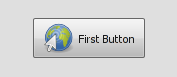
\includegraphics[width=\textwidth]{hello}
\end{center}
\end{frame}

\begin{frame}<presentation>
\begin{center}
Tobi Oetiker <tobi@oetiker.ch>
\end{center}
\end{frame}

\mode<article>{
\vspace{\stretch{1}}
Tobias Oetiker <tobi@oetiker.ch>
}
\end{document}

%%% Local Variables:
%%% TeX-master: "presentation.tex"
%%% mode: flyspell
%%% TeX-PDF-mode: t
%%% End:
